\documentclass[11pt,notitlepage]{article}

\usepackage[comma,numbers,sort&compress]{natbib}
\usepackage{graphicx}
\usepackage{color}
\usepackage{soul}
\usepackage{amssymb}
\usepackage{amsbsy}
\usepackage{theorem}
\usepackage{xcolor}
\usepackage{fullpage}
\usepackage{amsmath}
\usepackage{bm}
\usepackage{empheq}
\usepackage{centernot}
\usepackage{mathtools}
\usepackage{stmaryrd}
\usepackage[margin=1cm]{caption}
\usepackage{algorithmic}
\usepackage{helvet}
\renewcommand{\familydefault}{\sfdefault}
\usepackage[affil-it]{authblk}

\begin{document}

\section{Summary vision statement}
\subsection{Limitations and bottlenecks in the current state of the art}

\section{Project plan}
\subsection{Description of methodology to be used}
\subsubsection{Overview of reasoning engine}
We propose to implement a reasoning engine based on the formalism of Tractable
First-Order Probabilistic Logic and its associated Tractable Markov Logic (TLM)
language developed by \citet{Domingos:2012wi}. In keeping with the distributed
nature of Translator's Knowledge Sources, the reasoning engine that will
generate the dossier will operate on a Markov Logic Network learned from the
{\em schemas\/} and other metdata of Knowledge Sources; it will not be a network
of all biological interactions contained in the Knowledge Sources. The reasoning
engine's input will be a data structure representing the parsed natural language
query (see Sec.~\ref{sec:nlp}). The reasoning engine's output will be a {\em
  dossier,\/} i.e., a ranked list of {\em search strategies,\/} where a search
strategy is a possible joining of result-sets from one or more queries of
Translator Knowledge Sources (KS).

\subsubsection{Example to show how the reasoning engine will work}
We will illustrate the {\em search strategy\/} idea with a concrete
example. Suppose a user wishes to find a common mechanism to explain the
association of a variant $V$ with two different diseases $D1$ and $D2$
(Fig.~\ref{fig:networks}a).
\begin{figure}[h!]
  \begin{tabular}{cccc}
    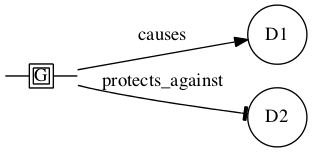
\includegraphics[width=1.4in]{baseproblem.png} &
    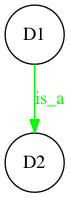
\includegraphics[width=0.35in]{net1.png} &
    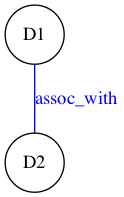
\includegraphics[width=0.6in]{net2.png} &
    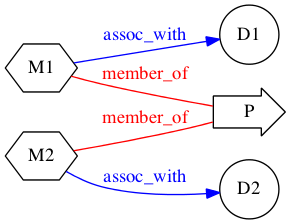
\includegraphics[width=1.5in]{net3.png}\\
    {\bf (a) Query} & {\bf (b) Search Strategy 1} & {\bf (c) Search Strategy 2} & {\bf (d) Search Strategy 3}
  \end{tabular}
  \caption{Example query predicate information (A) and examples of some simple
    search strategies (B--D) that would be examined by the reasoning engine based on
    a Markov Logic Network representing possible {\em types of connections\/}  between biological
    entities that are
   . Color denotes database to be searched (green: Disease Ontology,
    blue: DisGeNET, red: Pathway Commons). Black edges denote the query
    predicate variant-disease relationships. Circles denote the diseases D1 and
    D2, the boxed G denotes a variant, the large arrow shape denotes a pathway
    P, and hexagons denote the protein molecules M1 and M2 (or equivalently,
    their associated genes).}
  \label{fig:networks}
\end{figure}
A simple strategy would be to search to obtain a list of (disease,disease)
tuples representing ``is-a'' relationships from the Gene Ontology database
(Fig.~\ref{fig:networks}b) where the edge would be assigned a weight in the
Markov Logic Network based on the strength of evidence of this information type
(either a fixed weight for the database, or with more information, the weight
could be the ratio of prevalence of $D1$ to prevalence of $D2$). (We note that
this search strategy would not be selected by the reasoning engine because the
``is a'' relationship between two diseases is not consistent with the variant
being protective against disease D2 and causal for disease D1). An alternative
simple search strategy would be to load a list of {\em undirected\/}
$\{$disease,disease$\}$ pairs representing disease-disease associations from the
DisGeNET database (Fig.~\ref{fig:networks}c). An example of a {\em two}-database
search strategy would be to join (molecule,disease) ``associated\_with'' tuples
(from DisGeNET or Pharos) with (molecule,pathway) tuples representing
``member\_of'' relationships from Pathway Commons (Fig.~\ref{fig:networks}d). An
example of a {\em three}-database search strategy, for the same user query about
a variant-to-two-diseases association (Fig.~\ref{fig:threedb}a), is shown in
Fig.~\ref{fig:threedb}b.
\begin{figure}[h!]
  \begin{tabular}{ccc}
  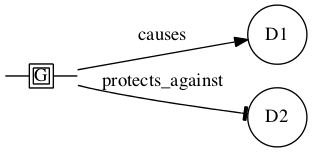
\includegraphics[width=1.4in]{baseproblem.png} &    
  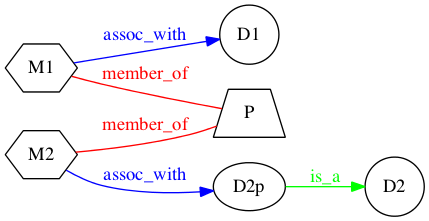
\includegraphics[width=2in]{net4.png} &
  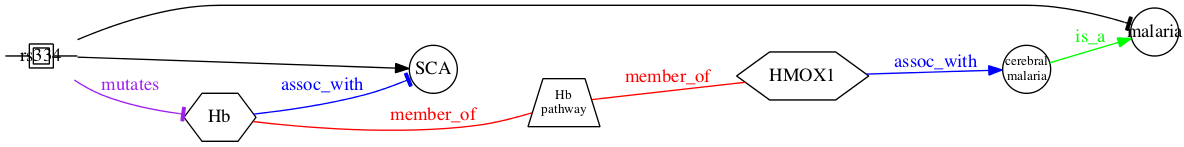
\includegraphics[width=2.5in]{net5.png} \\
                  {\bf (a) Query} & {\bf (b) Search Strategy 4} & {\bf (c) Search Result}
  \end{tabular}
  \caption{Example query predicate information (A); three-database example
    search strategy (B); matching search result for the specific query example
    G=rs334, D1=sicke-cell anemia (SCA) and D2=malaria (C). Edge color denotes
    the Knowledge Source to be searched (blue, DisGeNET; red, Pathway Commons;
    and green, Disease Ontology). Black edges denote the original query. Purple
    edge is the inferred interaction that explains the two black edges in light
    of the colored edges.}
  \label{fig:threedb}
\end{figure}
Let's assume that the variant G in this example query scenario is rs334, a
pleiotropic rare (MAF = 0.014\%) variant for which the homozygous minor allele
causes the blood disorder sickle-cell anemia (D1) and protects against malaria
(D2). The three-database search strategy shown in Fig.~\ref{fig:threedb}b would
yield a match indicating that a potential explanation for the pleiotropy of
rs334 is that it inhibits the hemoglobin pathway, thus reducing circulating
levels of free heme, which has been reported to be protective in the case of
cerebral malaria (a neurological complication of malarial
disease)~\cite{Ferreira:2011ff}.

\subsubsection{Composition of the Markov Logic Network}
We will use the Java-baesd (and open-source) NCATS-Tangerine Beacon Aggregator
to obtain metadata (schemas and entity counts) from Knowledge Sources via
RESTful queries leveraging the common Translator Knowledge Beacon Application
Programming Interface (KBAPI).


\subsection{Anticipated functionality for the POC reasoning tool}
\subsection{Components of the proposed software stack}

\subsubsection{Natural language query analyzer}
\label{sec:nlp}
Should we use the Stanford CoreNLP with BioNLP shared task data? If so, which
Python API should we use? (There are about a dozen of them).

\subsection{How proposed software will interact with Translator}

%% \section{Background: Types of questions}
%% \subsection{How does drug X induce clinical outcome Y?}
%% \subsection{Why do variants that cause sicke-cell anemia protect against malaria?}
%% \subsection{In people with variants found in any of the 22 known FA genes, is there increasing incidence of apalastic anemia
%%   (or other diseases)?}
%% \subsection{What venomous species have resulted in drugs approved by the FDA?}
%% \subsection{What cellular processes in which tissues are impacted in a patient-based EMR?}
%% \subsection{Why does ingestion of GlcNAc ameliorate symptoms of ngly1 deficiency?}

%% \section{Background: Knowledge Sources}
%% \begin{description}
%% \item[EBI String]{Protein-protein interactions}
%% \end{description}

\section{Personnel}

\bibliographystyle{plainnat}
\bibliography{conclett}

\end{document}
